%File: formatting-instructions-latex-2025.tex
%release 2025.0
\documentclass[letterpaper]{article} % DO NOT CHANGE THIS
\usepackage{aaai25}  % DO NOT CHANGE THIS
\usepackage{times}  % DO NOT CHANGE THIS
\usepackage{helvet}  % DO NOT CHANGE THIS
\usepackage{courier}  % DO NOT CHANGE THIS
\usepackage[hyphens]{url}  % DO NOT CHANGE THIS
\usepackage{graphicx} % DO NOT CHANGE THIS
\urlstyle{rm} % DO NOT CHANGE THIS
\def\UrlFont{\rm}  % DO NOT CHANGE THIS
\usepackage{natbib}  % DO NOT CHANGE THIS AND DO NOT ADD ANY OPTIONS TO IT
\usepackage{caption} % DO NOT CHANGE THIS AND DO NOT ADD ANY OPTIONS TO IT
\frenchspacing  % DO NOT CHANGE THIS
\setlength{\pdfpagewidth}{8.5in}  % DO NOT CHANGE THIS
\setlength{\pdfpageheight}{11in}  % DO NOT CHANGE THIS
%
% These are recommended to typeset algorithms but not required. See the subsubsection on algorithms. Remove them if you don't have algorithms in your paper.
\usepackage{algorithm}
\usepackage{algorithmic}

%
% These are are recommended to typeset listings but not required. See the subsubsection on listing. Remove this block if you don't have listings in your paper.
\usepackage{newfloat}
\usepackage{listings}
\DeclareCaptionStyle{ruled}{labelfont=normalfont,labelsep=colon,strut=off} % DO NOT CHANGE THIS
\lstset{%
	basicstyle={\footnotesize\ttfamily},% footnotesize acceptable for monospace
	numbers=left,numberstyle=\footnotesize,xleftmargin=2em,% show line numbers, remove this entire line if you don't want the numbers.
	aboveskip=0pt,belowskip=0pt,%
	showstringspaces=false,tabsize=2,breaklines=true}
\floatstyle{ruled}
\newfloat{listing}{tb}{lst}{}
\floatname{listing}{Listing}
%
% Keep the \pdfinfo as shown here. There's no need
% for you to add the /Title and /Author tags.
\pdfinfo{
/TemplateVersion (2025.1)
}

% DISALLOWED PACKAGES
% \usepackage{authblk} -- This package is specifically forbidden
% \usepackage{balance} -- This package is specifically forbidden
% \usepackage{color (if used in text)
% \usepackage{CJK} -- This package is specifically forbidden
% \usepackage{float} -- This package is specifically forbidden
% \usepackage{flushend} -- This package is specifically forbidden
% \usepackage{fontenc} -- This package is specifically forbidden
% \usepackage{fullpage} -- This package is specifically forbidden
% \usepackage{geometry} -- This package is specifically forbidden
% \usepackage{grffile} -- This package is specifically forbidden
% \usepackage{hyperref} -- This package is specifically forbidden
% \usepackage{navigator} -- This package is specifically forbidden
% (or any other package that embeds links such as navigator or hyperref)
% \indentfirst} -- This package is specifically forbidden
% \layout} -- This package is specifically forbidden
% \multicol} -- This package is specifically forbidden
% \nameref} -- This package is specifically forbidden
% \usepackage{savetrees} -- This package is specifically forbidden
% \usepackage{setspace} -- This package is specifically forbidden
% \usepackage{stfloats} -- This package is specifically forbidden
% \usepackage{tabu} -- This package is specifically forbidden
% \usepackage{titlesec} -- This package is specifically forbidden
% \usepackage{tocbibind} -- This package is specifically forbidden
% \usepackage{ulem} -- This package is specifically forbidden
% \usepackage{wrapfig} -- This package is specifically forbidden
% DISALLOWED COMMANDS
% \nocopyright -- Your paper will not be published if you use this command
% \addtolength -- This command may not be used
% \balance -- This command may not be used
% \baselinestretch -- Your paper will not be published if you use this command
% \clearpage -- No page breaks of any kind may be used for the final version of your paper
% \columnsep -- This command may not be used
% \newpage -- No page breaks of any kind may be used for the final version of your paper
% \pagebreak -- No page breaks of any kind may be used for the final version of your paperr
% \pagestyle -- This command may not be used
% \tiny -- This is not an acceptable font size.
% \vspace{- -- No negative value may be used in proximity of a caption, figure, table, section, subsection, subsubsection, or reference
% \vskip{- -- No negative value may be used to alter spacing above or below a caption, figure, table, section, subsection, subsubsection, or reference

\setcounter{secnumdepth}{0} %May be changed to 1 or 2 if section numbers are desired.

% The file aaai25.sty is the style file for AAAI Press
% proceedings, working notes, and technical reports.
%

% Title

% Your title must be in mixed case, not sentence case.
% That means all verbs (including short verbs like be, is, using,and go),
% nouns, adverbs, adjectives should be capitalized, including both words in hyphenated terms, while
% articles, conjunctions, and prepositions are lower case unless they
% directly follow a colon or long dash
\title{Solving ARC-Prize Problems with Search and Predicate Logic}
\author{
    Matthew Ellis
}
\affiliations{
    Georgia Institute of Technology
}

\begin{document}

\maketitle

% \begin{abstract}
% Lorem Ipsum Abstract
% \end{abstract}

% Uncomment the following to link to your code, datasets, an extended version or similar.
%
% \begin{links}
%     \link{Code}{https://aaai.org/example/code}
%     \link{Datasets}{https://aaai.org/example/datasets}
%     \link{Extended version}{https://aaai.org/example/extended-version}
% \end{links}

\section{Introduction}
This Autumn, Mike Knoop and Francios Chollet put up over a million dollars to entice the Artificial Intelligence community to find a new and creative solution to the problem of instilling AI models with basic reasoning and common sense. More specifically, they are looking to find ways of developing models that ``acquire new skills and solve open-ended problems'' \cite{arcprize}.

These ARC problems are represented by grids of colored squares. This way, the problems are not dependent on any specific language or culture. For any given problem, there is a set of training pairs and a test input. These training pairs include both the input and output grids, while the test only comes with an input and no output. The user/model must generate an output grid to pair with the test input.

There is no formal problem definition for any of these problems - an agent is simply supposed to examine the test pairs and deduce an output for the test input. For a human agent, this means using their intuition to recognize patterns or see a big picture that makes the answer readily apparent. However, computers struggle with these tasks as it is difficult to program a computer to handle an amorphous and vaguely defined task like this one.

\bigskip

The first hurdle an agent has to clear is deciding what size the output should be. For many problems, this means simply copying the size of the input grid. But for others, the size of the output could depend on latent information in the input grid itself.

Figure~\ref{fig:ex1} depicts a scenario where the output shape is the same as the input shape, but that is not the case for Figure~\ref{fig:ex2}.

\begin{figure}[htbp]
    \centering
    % First figure
    \begin{minipage}{0.22\textwidth}
        \centering
        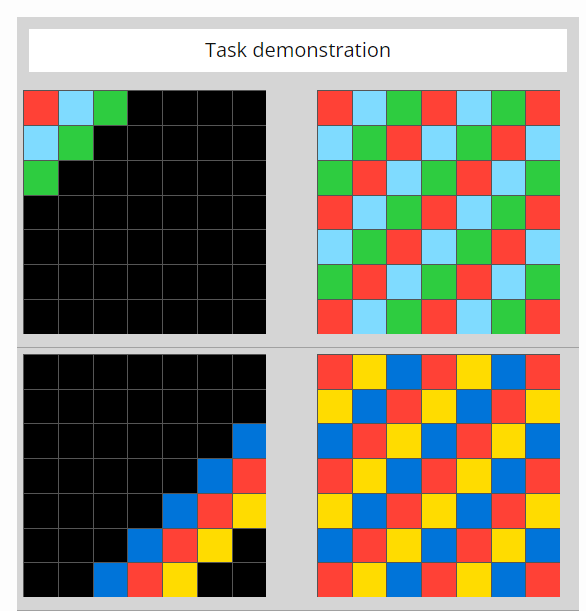
\includegraphics[width=\textwidth]{ex1.png}
        \caption{ARC Example}
        \label{fig:ex1}
    \end{minipage}
    \hfill
    % Second figure
    \begin{minipage}{0.22\textwidth}
        \centering
        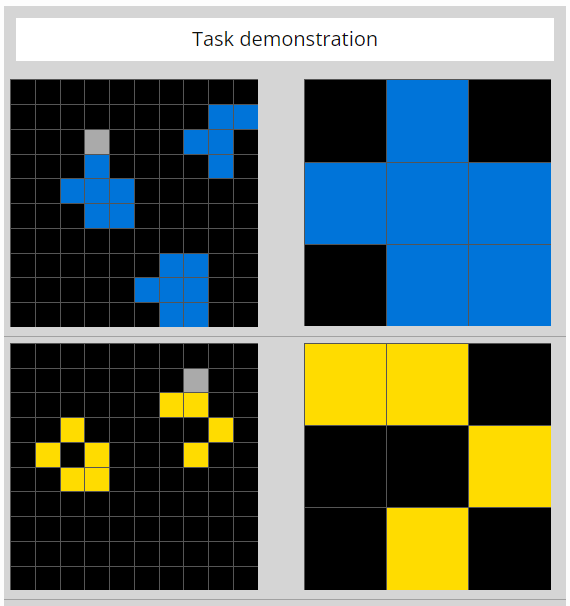
\includegraphics[width=\textwidth]{ex2.png}
        \caption{ARC Example}
        \label{fig:ex2}
    \end{minipage}
\end{figure}

Based on my experience solving a few of these puzzles, my basic workflow is
\begin{enumerate}
    \item Find a pattern between the size of the test inputs and their outputs (eg outputs are the same size as their inputs, shrunk by factor of 3, etc). Use this pattern to determine the test output size.
    \item Find a common pattern that maps the training inputs to their outputs.
    \item Apply this pattern to the test input to determine its output.
\end{enumerate}

\bigskip

In an effort to narrow the scope of the ARC problems a little bit, I classified some of the problems I saw into categories:


\begin{itemize}
    \item Binary Operation\\
    This is when the input is separated into 2 halves, and the output is the result of some binary operation (AND, XOR, \ldots) on these 2 halves. \\
    \item Stationary Input Modification\\
    This is when the output is nearly identical to the input except for a few squares being changed. All the 'structures' from the input remain in tact and in the same place.\\
    \item Dynamic Input Modification\\
    In these problems, the 'structures' remain in tact but move to other locations on the grid.\\
    \item Missing Window\\
    These problems include a square of uniform color sitting on top of a image, the goal being to determine what lies underneath the square. These can be solved using symmetry from other parts of the image.\\
    \item Downsampling\\
    The output grid is a smaller version of the input image, almost like a lower-level depiction of the same fractal.\\
    \item Upsampling \\
    The output grid is a larger version of the input image, almost like a higher-level depiction of the same fractal.\\
\end{itemize}

Knowing which class a problem falls into would make solving it much simpler; implementing functions to solve each of these problem classes individually would be simpler than implementing an algorithm to solve any ARC problem.

However, this would introduce a new problem of classifying a problem as one of the 6 above, which would be far from trivial in and of itself.

\bigskip

The more I learn about the ARC problems, the more I understand why Mike Knoop and Francios Chollet put such a large bounty on its solution. These are somewhat simple problems---simple to humans, at least---that have no good solution at the time of writing. It seems like an elegant solution to this problem \textit{has} to exist, but finding that solution won't be easy.

\section{Related Work}
Vanilla Machine Learning approaches and LLMs have both fallen well short of the human benchmark for ARC, so researchers have come up with creative ways of representing and solving these problems.

\bigskip

Xu, Khalil, and Stanner attempted to mimic the way humans think about ARC problems using Abstract Reasoning with Graphical Abstractions, or ARGA for short \cite{Xu_Khalil_Sanner_2023}. Their algorithm first transforms the grid of pixels into a graph of objects. These objects are clusters of pixels that humans would recognize as belonging together. Then, their algorithm can apply a transformation to these objects to modify the graph. These transformations are things like rotating an object, changing its color, removing it, etc. The algorithm searches through the state space of different combinations of these transformations until it reaches the output state. Then it simply applies these transformations to the test input grid.

To make this algorithm run in a reasonable amount of time, the search is optimized with a heuristic that selects the best state to expand on and constraints that limit the size of the search space. This approach was almost able to match the performance of the 2020 ARC Prize winner while using significantly less compute resources \cite{Xu_Khalil_Sanner_2023}.

\bigskip

Xu and Khalil also attempted to use LLMs to solve the ARC tasks. The first issue they ran into was representing the task grids as text, as LLMs like ChatGPT are primed to accept text input. This yielded poor results, so the researchers opted to use their ARGA generating algorithm from the paper mentioned above to feed ChatGPT an abstract graph instead of a concrete grid of text. This led to better performance, but their model didn't even reach 50\% accuracy on the easiest ARC problems \cite{xu2024llmsabstractionreasoningcorpus}.

\bigskip

Lee et al decided to go in a different direction - they tried using Reinforcement Learning to improve their model's analogical reasoning \cite{lee2024enhancinganalogicalreasoningabstraction}. They found that model-based RL yielded solid results, but with one major caveat. They restricted their action space to only 4 transformations plus a `submit' action in order to reduce compute complexity. Despite their promising results, it may be the case that RL isn't feasible to use on a problem as vast as the ARC Corpus.

\bigskip

Lei et al opted for yet another strategy: planning. They used the standard language for solving planning problems: Planning Domain Definition Language, or PDDL. Lei also used many strategies from Xu's 2023 paper, including abstract graph representation and argument constraints. Using this planning strategy, Lei was able to achieve an accuracy of over 50\% on the testing set, besting the previous winner's kaggle submission \cite{Lei_Lipovetzky_Ehinger_2024}.

\bigskip

In researching methods that others have used to solve the ARC problems, I also investigated some strategies around Raven's Progressive Matrices. The methods of solving these had some similar themes as the methods for solving ARC problems. Like strategies for solving ARC tasks, those for solving Raven's Progressive Matrices are composed of two main parts:
\begin{enumerate}
    \item Generate some higher-level representation of the information displayed in the problem.
    \item Infer a set of transformations and use them to deduce what the output should be.
\end{enumerate}
The paper I read about Raven's used a geometric approach to transformations, specifically affine transformations \cite{KUNDA201347}.

\bigskip

Throughout every paper I read, the key topics that kept popping back up were the 2 halves of the problem I mentioned immediately above. Multiple papers opted to solve the first half using the ARGA engine from Xu, Khalil, and Stanner 2023. This re-use of the ARGA engine leads me to believe that there is more room for improvement in step 2: transformation inference.

Thinking about the process of inferring transformations, I realized that many of the AI models in these papers perform poorly on the withheld testing set because the transformations in these tasks aren't appearing in the training set. A more robust AI model would be able to learn transformations as it goes instead of having the programmer hard code them into the source code. However, this is more easily said than done, and it may even be intractable with modern compute resources.

\section{Methodology}
My first attempt at solving the ARC Prize Problem was based on Breadth-First Search since this method is straightforward to implement and easy to understand. First, I had to find a Domain Specific Language for my algorithm to search over. I decided to reuse the actions from Homework 2 to build the DSL \cite{maclellan_arc_homework}. This DSL included only global actions---I did not implement any way to extract objects from the grids and search over object-specific actions. The actions that were encoded in the DSL are
\begin{itemize}
    \item tophalf
    \item rot90
    \item hmirror
    \item vmirror
    \item lshift
    \item compress
    \item mapcolor(a,b)
    \item trim
\end{itemize}
The pseudocode for my algorithm is described below:
\begin{algorithmic}
    \STATE $Q \gets initial \: state$
    \WHILE{$Q$ is not empty}
        \STATE $curr \: state \gets Q$.pop()
        \FORALL{$action$ $\in$ DSL}
            \STATE $new \: state \gets curr \: state$.perform$(action)$
            \IF{$new \: state = goal \: state$}
                \STATE Halt
            \ELSE
                \STATE $Q$.push$(new \; state)$
            \ENDIF
        \ENDFOR
    \ENDWHILE
\end{algorithmic}

\bigskip

I have also included the following visual representation of this algorithm in Figure~\ref{fig:algorithm}
\begin{figure}[htbp]
    \centering
    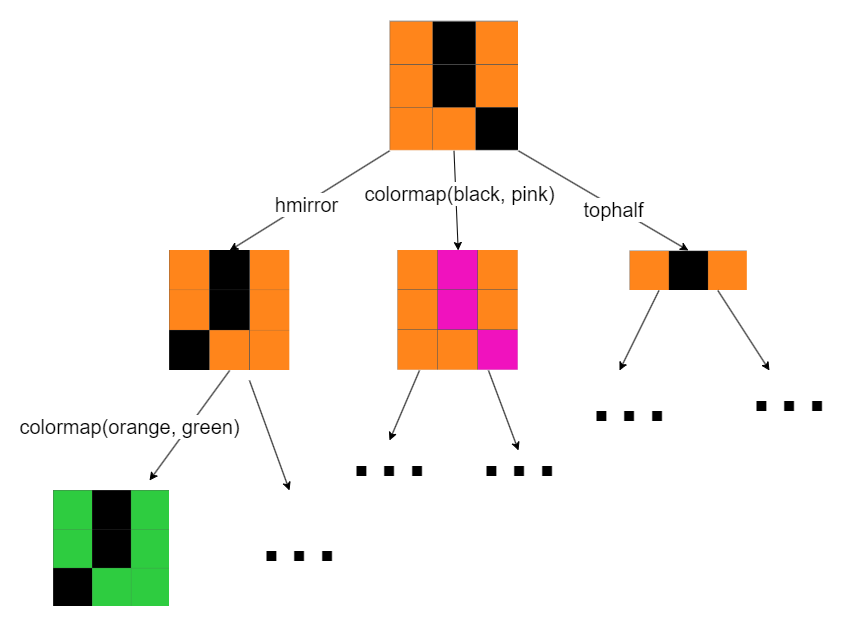
\includegraphics[width=\hsize]{BFS_tree.drawio.png}
    \caption{Search Algorithm Depiction}
    \label{fig:algorithm}
\end{figure}

\bigskip

This algorithm finds the chain of actions, which I will call the transformation, that transforms the initial state into the goal state. I also included a few optimizations in my implementation of this algorithm so that it would run in a reasonable amount of time.
\begin{itemize}
    \item Limit the depth of the search to 2 layers past the root
    \item Refuse to expand/revisit puzzle states that have already been added to the queue
    \item Only consider mapcolor($a$, $b$) if $a$ and $b$ actually show up in the input grid or output grid
\end{itemize}

\bigskip

Once the algorithm has inferred a transformation based on the training pair(s), it applies that transformation to the testing input(s) and submits the output. If the algorithm cannot infer a transformation that transforms the testing inputs into their respective outputs, then it infers the null transformation and simply returns the testing input(s) with no modifications.

\bigskip

If the algorithm infers multiple conflicting transformations from the training pairs, then it prefers to select the shorter transformation.

\bigskip\bigskip

For my second implementation, I attempted to improve on my original Breadth-First Search approach by introducing predicate logic. Specifically, each action could be conditioned on what colors are present in the grid at that time step. For example, my agent could learn a rule like


\begin{algorithmic}
    \IF{RED $\in grid$}
        \STATE mapcolor(RED, BLUE)
    \ELSIF{BLUE $\in grid$}
        \STATE mapcolor(BLUE, RED)
    \ELSE
        \STATE hmirror()
    \ENDIF
\end{algorithmic}

\bigskip

I implemented this by keeping track of the colors present in the grid at every state in the Breadth-First Search. This way, when the transformation for each training pair is found, that transformation also includes information about the colors at each step. From here, my agent builds a decision tree where, at each node, it decides on an action based on the colors present in the grid. This decision tree could look something like Figure~\ref{fig:tree}:

\begin{figure}[htbp]
    \centering
    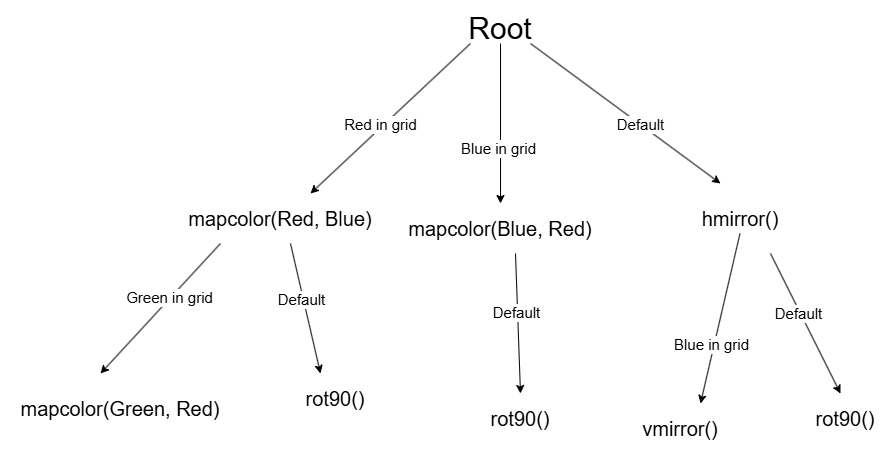
\includegraphics[width=\hsize]{decision tree.drawio.png}
    \caption{Decision Tree}
    \label{fig:tree}
\end{figure}

Once the decision tree has been constructed, the test input grid is passed through the decision tree, starting at the root. The specified actions are performed on it depending on what colors are present in the grid at each step, then it is submitted.

\section{Experiments}
Running my BFS algorithm without predicate logic yielded a score of 4 out of 400. I've included some ARC tasks that my algorithm was successfully able to solve below:

\begin{figure}[htbp]
    \centering
    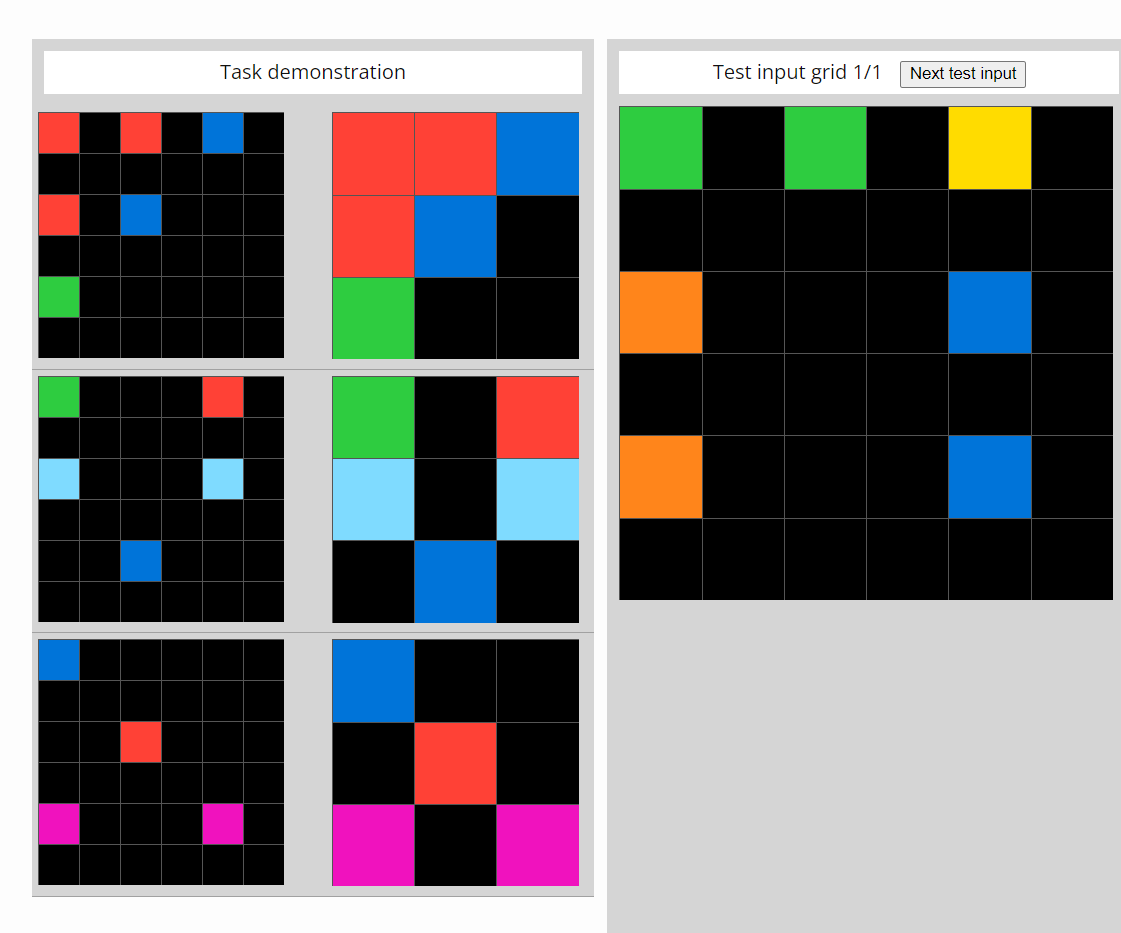
\includegraphics[width=0.8\hsize]{solved_1.png}
    \caption{Solved ARC Problem}
    \label{fig:solved_1}
\end{figure}
\begin{figure}[htbp]
    \centering
    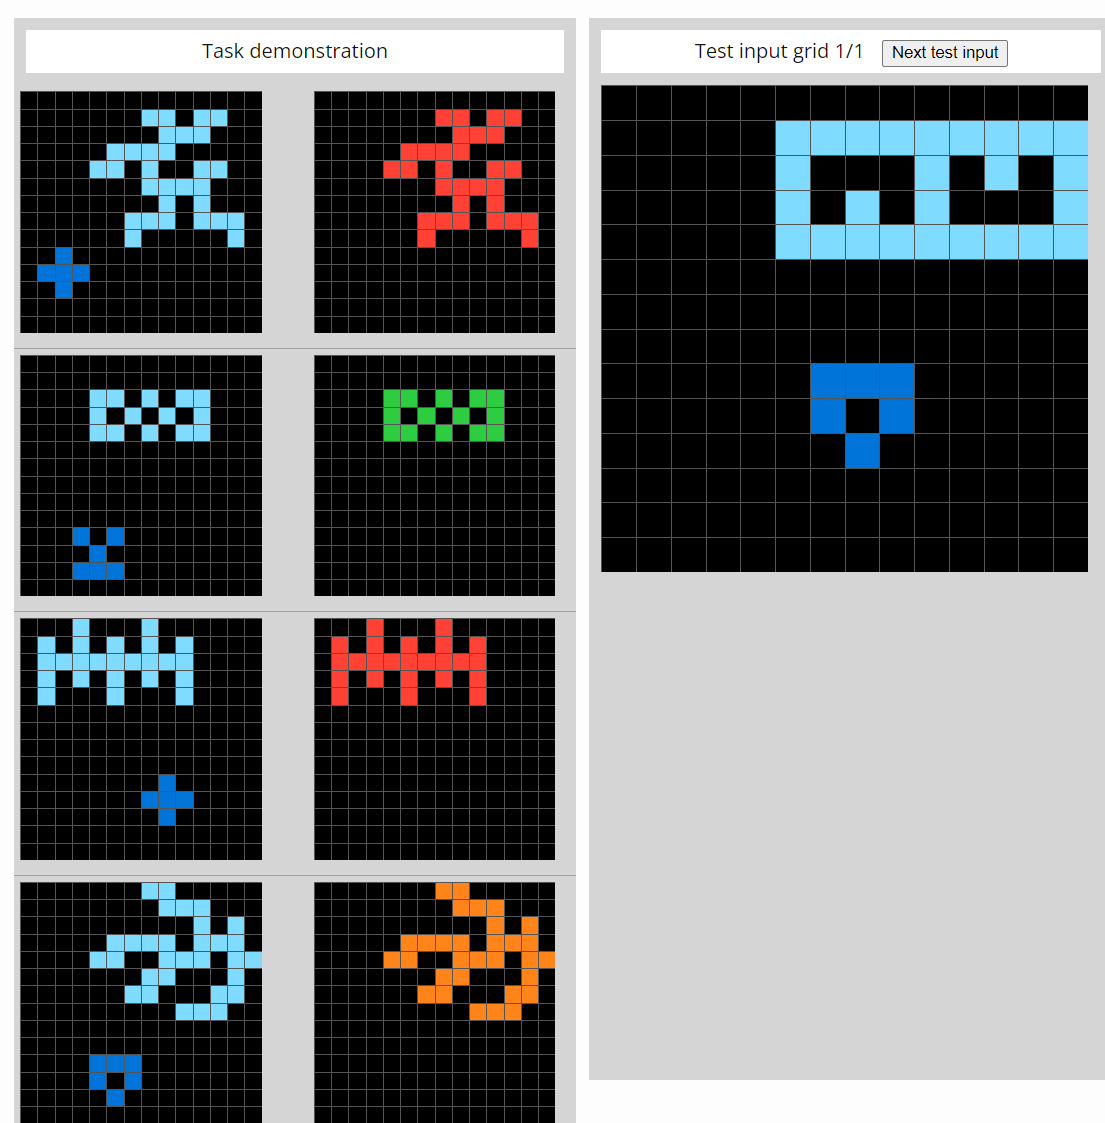
\includegraphics[width=0.8\hsize]{solved_2.png}
    \caption{Solved ARC Problem}
    \label{fig:solved_2}
\end{figure}
\begin{figure}[htbp]
    \centering
    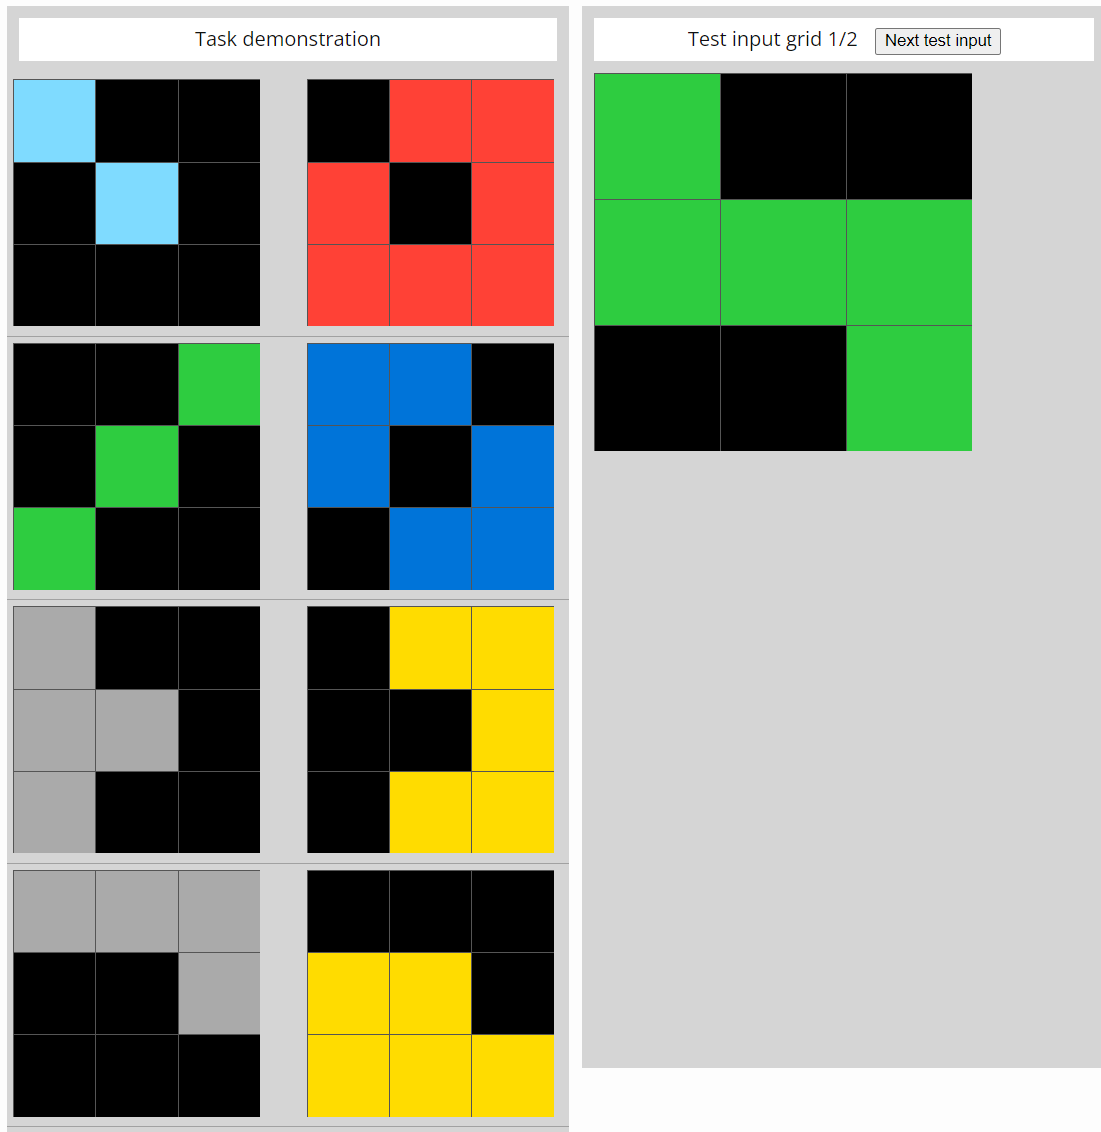
\includegraphics[width=0.8\hsize]{solved_3.png}
    \caption{Solved ARC Problem}
    \label{fig:solved_3}
\end{figure}
\begin{figure}[htbp]
    \centering
    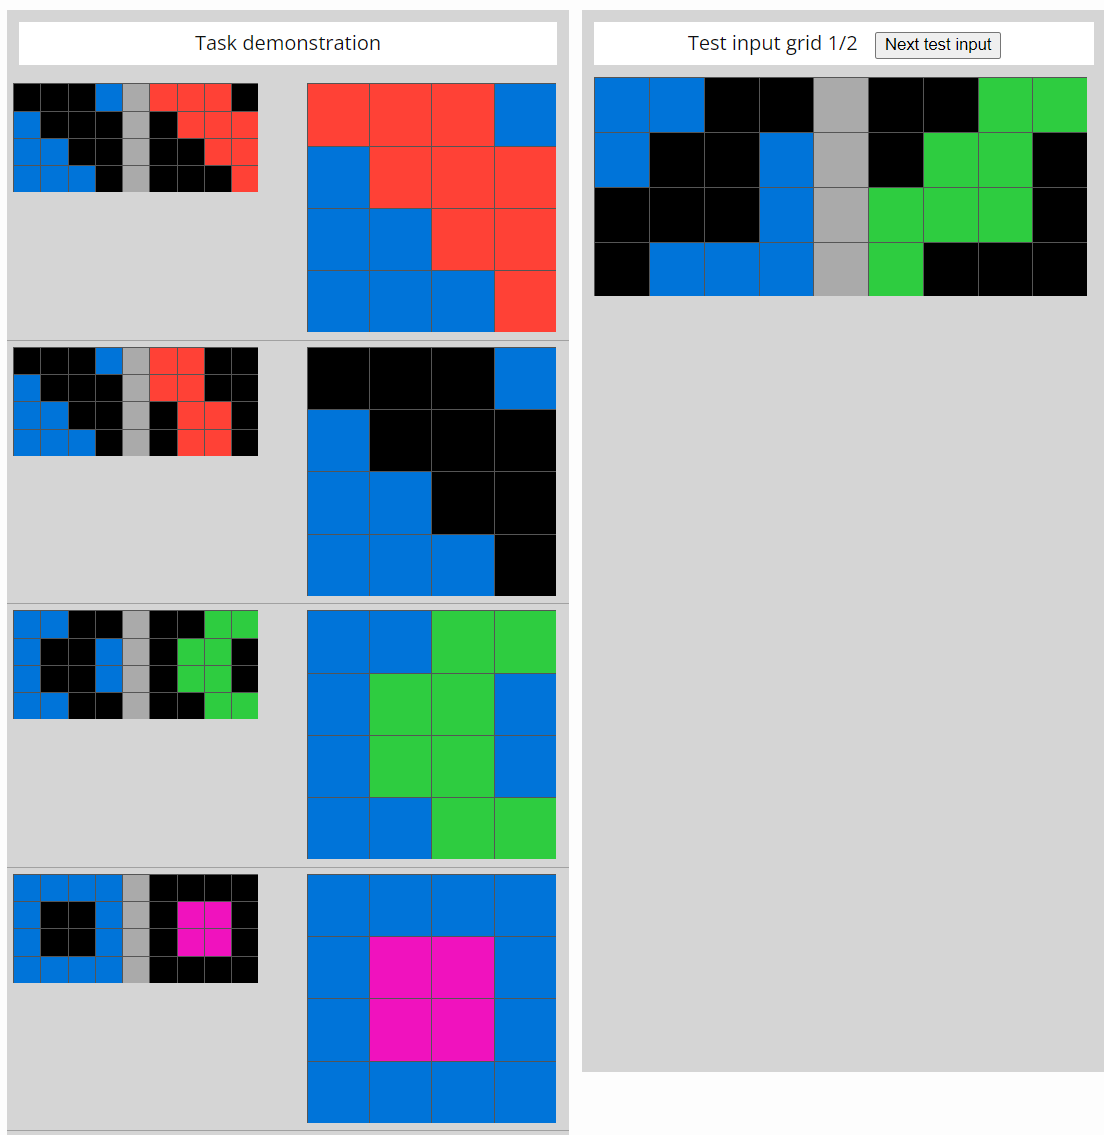
\includegraphics[width=0.8\hsize]{solved_4.png}
    \caption{Solved ARC Problem}
    \label{fig:solved_4}
\end{figure}

\bigskip

I will go over why my algorithm was able to solve these.

\bigskip

\noindent Figure~\ref{fig:solved_1}: This is a simple compression, which is defined in my DSL.

\bigskip

\noindent Figure~\ref{fig:solved_2}: This is a color mapping of dark blue to black, AND a complex color mapping that depends on the shape of the dark blue object in the input. My algorithm cannot infer this, so it must've made a lucky guess.

\bigskip

\noindent Figure~\ref{fig:solved_3}: The transformation here seems to be a compound color mapping, where black maps to different colors based on what color is shown in the input. My algorithm cannot infer this transformation, so it must've gotten lucky and inferred that black maps to blue, which would be correct for this test case.

\bigskip

\noindent Figure~\ref{fig:solved_4}: This is another transformation that my algorithm cannot infer, so it must've gotten lucky and arbitrarily used the 3rd training pair to infer a transformation of [ lhalf, colormap(black, green) ], which works for the given test input.

\bigskip

So my algorithm only functions properly for 1 out of 400 cases, but it sometimes gets lucky on another 3. This inspired my second implementation, as described in the Methodology section: the implementation with predicate logic.

\bigskip

However, my predicate logic implementation turned out to be less effective than my original implementation -- it scored a mere 2.5 out of 400,  only solving the problems in Figures~\ref{fig:solved_1}, \ref{fig:solved_3}, and \ref{fig:solved_4}. Despite predicate logic's ability to more accurately infer the semantics of problems like the ones in Figures~\ref{fig:solved_3} and \ref{fig:solved_4}, it was unable to solve the problem in Figure~\ref{fig:solved_2}, and it did not solve any new problems that my first attempt left unsolved.

\section{Results}

\renewcommand{\arraystretch}{1.5} % Increase row height
\setlength{\tabcolsep}{10pt}      % Increase column spacing

\begin{table}[H]
    \centering
    \resizebox{\columnwidth}{!}{ % Scale the table to fit within a column
    \begin{tabular}{|p{0.25\columnwidth}|c|c|} % Fixed-width first column
        \hline
        \textbf{Agent} & \textbf{Number Correct} & \textbf{Proportion Correct} \\
        \hline
        Vanilla BFS & 4 & 1\% \\
        \hline
        BFS and Predicate Logic & 2.5 & 0.6\% \\
        \hline
    \end{tabular}
    }
    \caption{Results Table}
\end{table}

Of the four `Solved ARC Problem' figures above, Figures~\ref{fig:solved_3} and \ref{fig:solved_4} can both be solved more reliably by noticing the correlation between the colors in the input and the colors in the output. For Figure~\ref{fig:solved_3}, it is clear that light blue implies a mapping of black to red, green implies a mapping of black to dark blue, and so on.

\bigskip

My original Breadth-First Search agent got the problems in Figures~\ref{fig:solved_3} and \ref{fig:solved_4} correct, but only with the help of some luck -- my agent wasn't able to infer the correct semantics here. These lucky guesses led me to believe that there were many more problems like these two in the ARC corpus that my agent was missing because it wasn't getting so lucky. Maybe I could solve more of these problems by inferring the conditional color mapping instead of relying on luck.

\bigskip

But this was not the case. My predicate logic agent scored a mere 2.5 out of 400, marking a decrease in performance from my original implementation.

\bigskip

My predicate logic implementation was able to solve the problems depicted in Figures~\ref{fig:solved_1}, \ref{fig:solved_3}, and \ref{fig:solved_4}, but not Figure~\ref{fig:solved_2}. I assume this is because the color transformation for Figure~\ref{fig:solved_2} is predicated on shape, not color.

\bigskip

Contrary to my expectations, my predicate logic implementation did not capture any additional problems from the ARC corpus that my first approach wasn't already capturing. I believe this is because there aren't that many problems in the ARC corpus that rely on simple, global transformations and color mappings.

\begin{figure}[htbp]
    \centering
    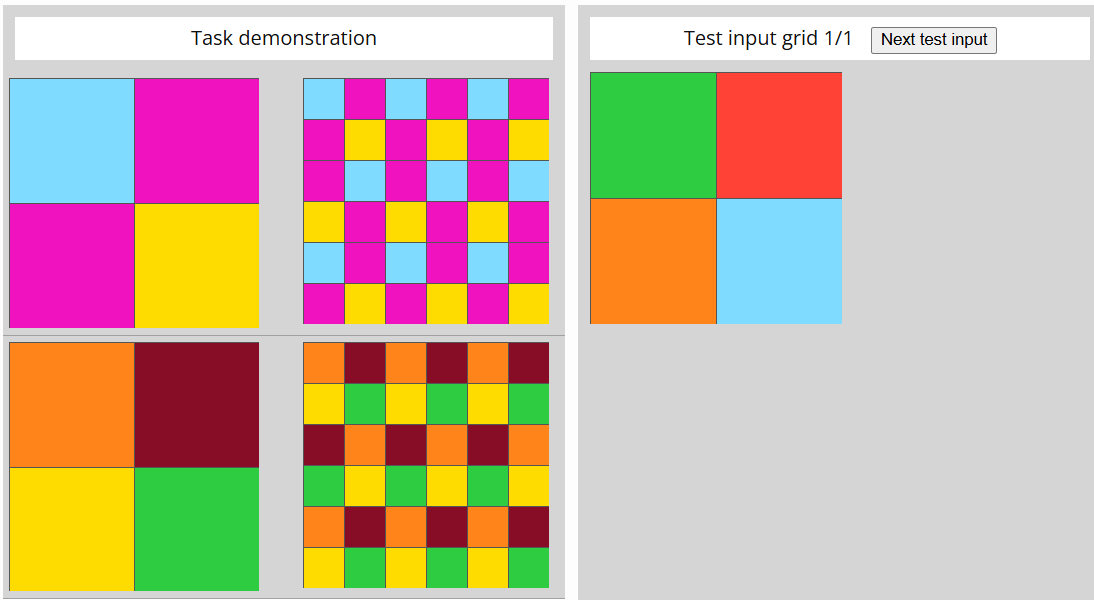
\includegraphics[width=\hsize]{unsolved.png}
    \caption{Unsolved ARC Problem}
    \label{fig:unsolved}
\end{figure}

\bigskip

I have included one last example ARC problem in Figure~\ref{fig:unsolved} to reinforce my claim that many ARC problems cannot be solved with global transformations and color mappings. 

\bigskip

Neither of my two agents were able to solve the problem in Figure~\ref{fig:unsolved} because it involves increasing the size of the output grid and tiling the input grid across the larger output grid. This behavior cannot be captured using global transforms, nor can it be predicated on colors that appear in the inputs. This is just one example of a type of problem that my agent isn't anywhere close to being able to solve, and it shows that predicating on color alone isn't nearly enough to realize the complex transformations endemic to the ARC corpus.


\section{Discussion}
My work here was inspired by Xu, Khalil, and Stanner's 2023 paper about inferring transformations from the training grids to apply to the test grid. Similar to my approach, they search over a space of potential actions, looking for the series of actions that will transform the training input into its respective training output \cite{Xu_Khalil_Sanner_2023}.

\bigskip

However, our approaches differ in the type of actions being searched over. My agent searches over global actions, while Xu's agent searches over object-specific transformations. I elected to search over global transformations so that I could keep my implementation fast, straightforward, and human-interpretable from top to bottom. There are no nebulous neural nets or latent parameters in my code, unlike Xu's approach which uses Abstract Reasoning with Graphical Abstractions, or ARGA for short.

\bigskip

I was hoping to discover that Xu missed something -- that maybe predicating actions based on color was a good enough heuristic to estimate object-specific transformations. This turned out to not be the case; object recognition seems to be a critical component of reliably solving ARC problems.

\bigskip

I believe that the strategies I've implemented here in this paper can play a part in an agent that can reliably solve ARC problems, but only a small part. A reliable agent would have to be able to recognize patterns, reason globally, reason at the object level, and reason over the relationships between the objects. On top of this, it would have to be able to do all that in a reasonable amount of time.

\section{Conclusion}
In conclusion, my model did not work as well as I would have liked. Breadth-First Search was able to correctly answer only 4 out of 400 ARC Prize Problems. To make matters worse, BFS only correctly `understood' the semantics of 1 transformation. The other 3 problems that my model got correct were essentially lucky guesses.

\bigskip

However, this lack of success tells another story: a tree search algorithm can be the engine behind a solid ARC Problem solver. My work here proves the concept that Breadth-First Search can reason over a set of transformations to determine a path from input to output. A more robust DSL of nuanced transformations could capture a much larger state space, which would cover more ARC Prize problems.

\bigskip

My model's ability to guess correctly on those 3 problems where it inferred the wrong transformation also tells another story. Tree searching algorithms like mine will be biased towards the simplest transformation between input and output. This inferred transformation might not capture all the nuances of the ground-truth transformation, but if it can capture some of the nuance, it has the ability to make an educated guess about the output. This ability to make educated guesses is another strength of tree search algorithms. The ARC Prize's hidden evaluation set contains many transformations that may be unfamiliar to the submitted bots and their creators, so it is important for the submitted bots to have the ability to take a stab at answering tough questions instead of simply throwing their hands up in defeat.

\bigskip

My biggest disappointment in this project was the lack of performance I encountered when implementing my predicate logic feature. As I mentioned earlier, my vanilla BFS implementation had a tendancy to over-generalize, so using predicate logic to infer more complex transformations seemed like an easy fix. Unfortunately, this instead lead to the problem of over-specifying --- my model would infer connections that simply didn't exist. This lead me to the conclusion that it is better to err on the side of general transformations rather than specific transformations. 

\bigskip

My model worked exactly as intended for at least one of the ARC Prize problems, which shows that there is some promise to the tree-search strategy. Search's ability to filter out red herrings by finding the shortest path from the initial state to the goal helps to distill the ARC Prize Problems to a simpler version of themselves, but one has to be careful to not loose too much of that detail. I couldn't quite strike the balance between specificity and generalization in my implementation, but my results show that Search can be a critical part of a performant ARC agent.

\section{Future Works}
As I mentioned in the Conclusion, one improvement that could be made to my work here is to build a more robust DSL of actions so that a search algorithm can infer more nuanced transformations. This DSL should include object-specific transformations, which would mean the inclusion of a method to recognize and abstract objects. Xu, Khalil, and Stanner's implementation was similar to this, but it might be improved on with tuning to the generality/specificity of the output \cite{Xu_Khalil_Sanner_2023}. One could make a search model more general by including broader heuristics or limiting the search depth, or more specific by predicating transformations like I attempted to do. 

\bigskip

One issue that may arise with a more nuanced DSL is runtime. My model's runtime started to get intractable when I tried to search a depth of more than 3 actions across my relatively limited DSL. One way to ameliorate this would be through informing the search algorithm with a heuristic instead of using vanilla BFS.

\bigskip

It now seems clear to me that a good solution to the ARC Prize Problem must include many separate subsystems all working in concert to synthesize a transformation, which is a bit frustrating to me. ARC problems are so elegant and simple --- they are just a pair of grids connected by latent pattern. Compared to other computer science problems like traveling salesman and encryption, the ARC problems almost look easy at first glance; they almost look like they should have a simple and straightforward solution, but it is clear to me now that this is not the case. A solution to the ARC Prize Problems won't come from some eureka moment or simple new algorithm, but instead from the meticulous integration of already-know AI algorithms into a seamless super-system.

\bibliography{sources}

\end{document}
